\chapter{Method}
%just some stuff for the sphere in the cube graphic
\tikzset{
    MyPersp/.style={scale=1.8,x={(-0.8cm,-0.4cm)},y={(0.8cm,-0.4cm)},
    z={(0cm,1cm)}},
   MyPoints/.style={fill=white,draw=black,thick}
    }
    
für die reproduzierbarkeit der BA \newline
was habe ich wie gemacht -> warum habe ich es so gemacht

In order to get familiar with this topic I first needed some background knowledge. To receive this knowledge I did use keyword searches on 'GoogleScholar' and then read the papers I found about the topic. To solve the problem, I also needed knowledge about \ac{CC3D}. I received this by reading their manuals and by trying out different settings, since there is no detailed documentation about their simulation.

To analyze the simulation scripts I used papers and a pen. Since, in this project it is not possible to use a compiler to debug the scripts, because the computation is done by \ac{CC3D}, to draw the the different function calls per hand was one of two ways to understand the scripts. The second way was to use print commands, i.e. an ouput at the console (another i.e.), to see at which point which function in which script is called. 


For this bachelor thesis I used a constructive research, i.e. develop a solution to a given problem.

\section{Draw Cells}
Since the program so far draws cubic cells and overgives the same parameter three times, a modification for this function was necessary. In the following the function call and the method of the old cell drawing method are displayed.
\begin{lstlisting}[language=Python, caption = function call of the cell drawing method addCubicCell for a 3D cell]
self._addCubicCell(2, xPos, 2, zPos, cellDiameter, cellDiameter, cellDiameter, steppable)
\end{lstlisting}
\begin{lstlisting}[language=Python, caption = method to draw cubic cells]
    def _addCubicCell(self, typename, xPos, yPos, zPos, xLength, yLength, zLength, steppable):
        cell = steppable.newCell(typename)
        xPosDim = self.execConfig.calcPixelFromMuMeter(xPos)
        yPosDim = self.execConfig.calcPixelFromMuMeter(yPos)
        zPosDim = self.execConfig.calcPixelFromMuMeter(zPos)
        xLengthDim = self.execConfig.calcPixelFromMuMeter(xLength)
        yLengthDim = self.execConfig.calcPixelFromMuMeter(yLength)
        zLengthDim = self.execConfig.calcPixelFromMuMeter(zLength)
        # size of cell will be SIZExSIZEx1
        steppable.cellField[xPosDim:xPosDim + xLengthDim - 1,
        					 yPosDim:yPosDim + yLengthDim - 1,
        					 zPosDim:zPosDim + zLengthDim - 1] = cell
\end{lstlisting}
In the function 'addCubicCell' the parameters are converted into pixels, using the 'calcPixelFromMuMeter' function and then the cube will be drawn. To provide a deeper understanding of the of \ac{CC3D} provided method, to draw the cell, the boundaries for the cube are displayed more generell in the following listing:
\begin{lstlisting}[language=Python, caption = boundaries of a drawn cuboid]
    steppable.cellField[xStart:xEnd,
    					 yStart:yEnd,
    					 zStart:zEnd] = cell
\end{lstlisting}        		
In the listing above x,y,zStart defines the start and x,y,zEnd the end point of the to drwan area for each axis.\newline
In order to be able to draw a cell as a sphere, \ac{CC3D} has to be able to draw all the different pixels containing to one cell. Because \ac{CC3D} allows the user to draw several pixels containing to one cell, a solution for this problem is possible.
It is possible to lay a cuboid around the sphere, as it is displayed in fiugre \ref{tikz:SphereInCube} at page \pageref{tikz:SphereInCube} and then decide if a point of the cuboid is in the sphere or not.
\begin{figure}
\begin{center}
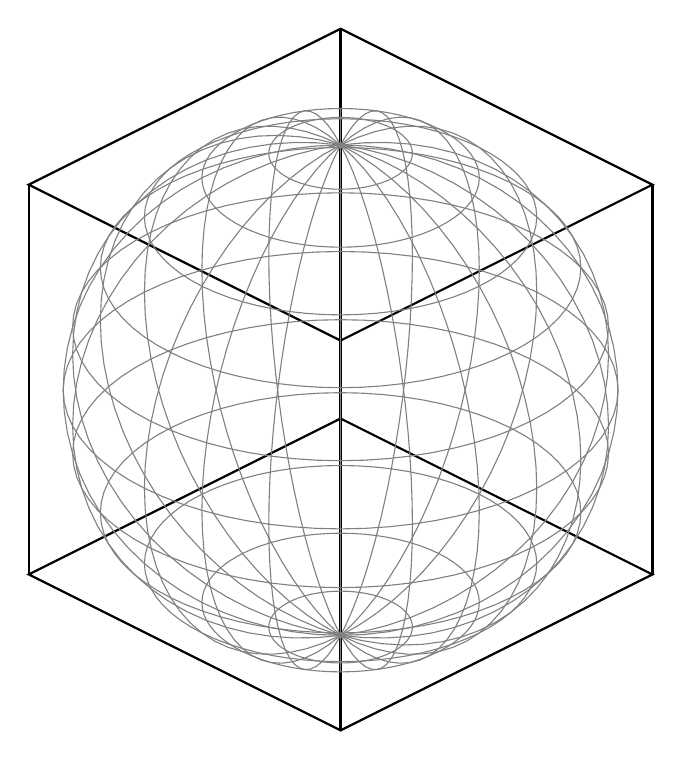
\begin{tikzpicture}[MyPersp,font=\large]%[scale=3]
%draw the three axis
%\draw[thick,->] (0,0,0) -- (3.0,0,0) node[anchor=north east]{$x$};
%\draw[thick,->] (0,0,0) -- (0,3.0,0) node[anchor=north west]{$y$};
%\draw[thick,->] (0,0,0) -- (0,0,3.0) node[anchor=south]{$z$};

\draw[black,thick] (0,0,0) -- (0,2.75,0) -- (2.75,2.75,0) -- (2.75,0,0) -- cycle;
\draw[black,thick] (0,0,2.75) -- (0,2.75,2.75) -- (2.75,2.75,2.75) -- (2.75,0,2.75) -- cycle;
%
%%draw the edges of the cube
\draw[black,thick] (0,0,0) -- (0,0,2.75);
\draw[black,thick] (0,2.75,0) -- (0,2.75,2.75);
\draw[black,thick] (2.75,0,0) -- (2.75,0,2.75);
\draw[black,thick] (2.75,2.75,0) -- (2.75,2.75,2.75);

\foreach \t in {0,15,...,150}% meridians
    {\draw[gray] ({1.73*cos(\t)+1.0},{1.73*sin(\t)+1.0},1.0)
        \foreach \rho in {5,10,...,360}
            {--({1.73*cos(\t)*cos(\rho)+1.0},
 			{1.73*sin(\t)*cos(\rho)+1.0},{1.73*sin(\rho)+1.0})}--cycle;
    }
\foreach \t in {-75,-60,...,75}% parallels
   {\draw[gray] ({1.73*cos(\t)+1.0},1.0,{1.73*sin(\t)+1.0})
        \foreach \rho in {5,10,...,360}
           {--({1.73*cos(\t)*cos(\rho)+1.0},   
			{1.73*cos(\t)*sin(\rho)+1.0},{1.73*sin(\t)+1.0})}--cycle;
   }  
\end{tikzpicture}
\caption{A cuboid layed around a sphere}
\label{tikz:SphereInCube}
\end{center}
\end{figure}

As long as both, the cuboid and the sphere, have the same center it is possible to calculate every point inside or outside the sphere\cite{REF}. To do so, for every point within the cuboid it is necessary to calculate if the distance to the center is smaller or equal to the radius of the sphere. If this is the case, the point is inside of the sphere, otherwise it is outside of the sphere. Thus, the formula to determine if a point is inside of the sphere is the following:
\begin{equation}
\sqrt{(x_{r}-x_{0})^2 + (y_{r}-y_{0})^2 + (z_{r}-z_{0})^2} <= radius
\end{equation}
In this formula $x_{r},y_{r},z_{r}$ contains the current point of the specific axis and $x_{0},y_{0},z_{0}$ is the center of the cuboid and the sphere. Whenever the distance of the current point in the cuboid to the center is smaller or equal the radius of the sphere, than this point is inside of the sphere. \newline
In order that it is possible to draw the cells in this way, the iteration over all points of the cuboid is necessary. Because to do this is computational more expensive than to just draw a cube, the cuboid should be as small as possible. Still, the cuboid has to be at least as large as $2*radius$ of the sphere, as it is displayed figure \ref{tikz:CuboidSphere} at page \pageref{tikz:CuboidSphere}.
\begin{figure}
\begin{center}
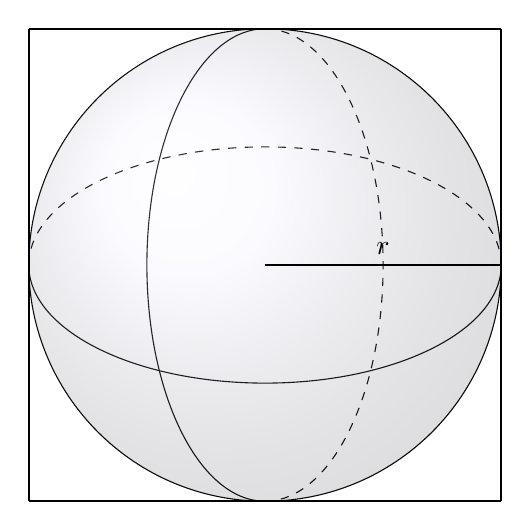
\begin{tikzpicture}[scale=3]
    \draw (-1,0) arc (180:360:1cm and 0.5cm);
    \draw[dashed] (-1,0) arc (180:0:1cm and 0.5cm);
    \draw (0,1) arc (90:270:0.5cm and 1cm);
    \draw[dashed] (0,1) arc (90:-90:0.5cm and 1cm);
    \draw (0,0) circle (1cm);
    \shade[ball color=blue!10!white,opacity=0.20] (0,0) circle (1cm);
    \draw[thick] (0,0) -- node[above]{$r$} (1,0);
    %\draw[thick] (0,0) -- node[above]{$rd$} (-.7,-.7);
  
%\draw[blue,thick] (0,0,0) -- (0,2.75,0) -- (2.75,2.75,0) -- (2.75,0,0) -- cycle;
%\draw[blue,thick] (0,0,2.75) -- (0,2.75,2.75) -- (2.75,2.75,2.75) -- (2.75,0,2.75) -- cycle;
%
%%draw the edges of the cube
\draw[black,thick] (-1,-1) -- (1,-1);
\draw[black,thick] (-1,-1) -- (-1,1);
\draw[black,thick] (-1,1) -- (1,1);
\draw[black,thick] (1,-1) -- (1,1);
\end{tikzpicture}
\caption{A cuboid with minimal size layed around a sphere}
\label{tikz:CuboidSphere}
\end{center}
\end{figure}


Since we need the old method to draw the basal membrane throughout the whole area, a new function is required. The old function is refactored into 'addMembrane', i.e. renamed and every time the function name appears within the project, within a comment or the function is called, this appearance is also change. With the new method name it clear that this function is now, in the 3D simulation, only required for the basal membrane, since it is a cubic cell, and if some simulations in two dimensions are made.\newline
The created function 'add3DCell', it is displayed in the listing below, is similiar to the old one, as it also has to convert the used points, i.e. the start and end point of the cuboid and the center of the cuboid and the sphere, into pixels. Then the iteration of all three axis as well as the calculation to decide if the pixel is inside the sphere or not takes place.

\begin{lstlisting}[language=Python, caption = created method to draw a spere cell]
    def _add3DCell(self, typename, xPos, yPos, zPos, radius, steppable):
        '''The parameters are all in micro meter
        wheras the calculated variables are in px'''

        cell = steppable.newCell(typename)
        xStart = self.execConfig.calcPixelFromMuMeter(xPos - radius)
        x0 = self.execConfig.calcPixelFromMuMeter(xPos)
        xEnd = self.execConfig.calcPixelFromMuMeter(xPos + radius)
        yStart = self.execConfig.calcPixelFromMuMeter(yPos - radius)
        y0 = self.execConfig.calcPixelFromMuMeter(yPos)
        yEnd = self.execConfig.calcPixelFromMuMeter(yPos + radius)
        zStart = self.execConfig.calcPixelFromMuMeter(zPos - radius)
        z0 = self.execConfig.calcPixelFromMuMeter(zPos)
        zEnd = self.execConfig.calcPixelFromMuMeter(zPos + radius)

        radiusPx = self.execConfig.calcPixelFromMuMeter(radius)

        for xr in range(xStart, xEnd):
            for yr in range(yStart, yEnd):
                for zr in range(zStart, zEnd):
                    rd = sqrt((xr - x0) ** 2 + (yr - y0) ** 2 + (zr - z0) ** 2)
                    if (rd <= radiusPx):
                        steppable.cellField[xr, yr, zr] = cell
\end{lstlisting}

With this created function it is now possible to draw a cell as a sphere, as it is displayed at figure XY \cite{XY}. This has several advantages, as we are now able not to increase the $\lambda_{sur}$ in a way that the volume constraint does not count as it will be really consider..........................

\section{Lambda Multiplier}
In the project there were several places, where a lambda multiplier for the effective energy, see section 1.X, is calculated, but it is only set once. There are two additional multipliers, for the surface and volume constraints, saved in within each cell object. Since we are not using these values in the programm and they do not influence or set the $\lambda_{vol}$ or $\lambda_{sur}$ which \ac{CC3D} uses, these two values were outcommented in the first step and later deleted. \newline 
Also in one place there were methods to calculate the lambda values. Since this methods are not used in the project and moreover they had a multiplier itself to calculate the multiplier for the specific effective energy, as it is displayed in the following listing, these were also first outcomented and later deleted.
\begin{lstlisting}[language=Python, caption= methods to calculate the $\lambda_{vol}$ and $\lambda_{sur}$ for the effective energy]
    def calcSurLambdaFromSurFit(self, surFit):
        return 100.0 * surFit

    def calcVolLambdaFromVolFit(self, volFit):
        return 1.0 * volFit
\end{lstlisting}

In the project the multipliers for the effective energy are now set each time when a cell is initialized. A second time the multiplier $\lambda_{vol}$ is set, is during necrosis, in generell if a cell dies. Thus, there is now the advantage that at a specific point in the coding these values are set.




\section{Approximation Error}
Since the project includes conversions from \SI{}{\micro\metre} to pixels and the amount of pixels, e.g. for the surface of a cell, have to be set in integer, i.e. a whole number, it is possible that in some places in the program there are approximation errors. In the project, the values of \SI{}{\micro\metre} are saved either with the data type double or float -- both allow several decimal digits. To set these values as a whole number the values are casted, i.e. the datatype of a variable, i.e. a placeholder, will be changed -- in this context the values of type double or float will be transformed to a whole number by cutting of the decimal digits. At some points in the project the values of \SI{}{\micro\metre} are converted to a whole number and then it is further calculated with this casted value. To cast the value should always be the last step in order to avoid approximation and calculation errors. In the following listings an example of to early casting is displayed:

\begin{lstlisting}[language=Python, caption=example of an calculation error because of an too early executed cast]
    def calcVoxelVolumeFromVolume(self, volume):

        r = (3 * volume / (4.0 * PI)) ** (1.0 / 3.0)  # Radius of a sphere with known volume.
        rDimension = self.calcPixelFromMuMeter(r)  # Convert it to a pixel unit.
        
        if self.dimensions == 2:
            return self.__truncate(PI * (rDimension ** 2))  # Area of a circle.
        else:
			return self.__truncate(4.0 / 3.0 * PI * (rDimension ** 3)) # Volume of a sphere.
\end{lstlisting}
\begin{lstlisting}[language=Python, caption=function to convert values of \SI{}{\micro\metre} into pixel]
    def calcPixelFromMuMeter(self, mum):
		return int(self.voxelDensity * mum + 0.000001)
\end{lstlisting}

In this example the second command of the 'calcVoxelVolumeFromVolume' function calls the function of the second listing, in which the approximation error happen. Since the decimal digits are just cut off, the further calculation contains a wrong value and as a consequence the result of the calculation is incorrect. \newline
In order to solve the problem the complete calculation is calculated with decimal digits. After the calculation is done it will be checked if the first decimal digit is larger or equal to 5. If this condition is true the result is increased by 1 otherwise not, as a last step the result is casted. This technique has the advantage that calculation errors due to casting are decreased, because the cast is the very last step. It is possible that in the program still have some rounding errors, but these are not as dramatic as an casting error in the calculation. To remove this casting error, the function 'calcVoxelVolumeFromVolume' is extended in the following way.

\begin{lstlisting}[language=Python, caption = the same function as before but without approximation errors\, because the cast and the rounding is done after the calculation]
   def calcVoxelVolumeFromVolume(self, volume):
        r = (3 * volume / (4.0 * PI)) ** (1.0 / 3.0)  # Radius of a sphere with known volume.
        rDimension = r * self.voxelDensity
        if self.dimensions == 2:
            return int(self.__truncate(PI * (rDimension ** 2)))  # Area of a circle.
        else:
            result = 4.0 / 3.0 * PI * (rDimension ** 3)
            if result % 1.0 >= 0.5:
                result += 1

            return int(result)
\end{lstlisting}

One use of the function is to calculate the volume constraints of a specfic cell type. In the simulation a minimum and a maximum volume for each cell type is calculated by the function 'calcVoxelVolumeFromVolume'. These value are used in the calculation to determine if mitosis takes place or not. \newline
For the basal cell the minimum volume is \SI{381}{\micro\metre} and the maximal volume is \SI{523}{\micro\metre}. With the old calculation the minimum volume constraint would be the same as for the stem cells --905vx. Since the current calculation only casts and round at the very last step, the result is now 1286vx, which is a more precise and correct result. In the following table \ref{tbl:Approximation error} an example of to early rounding and casting is displayed:

\begin{table}[h]
\centering
\caption{Stakeholders' motivations to use \ac{SW CS}}
\renewcommand{\arraystretch}{1.5}
	\begin{tabularx}{\textwidth}{XXXXX}
		Volume in \SI{}{\micro\metre} & radius in \SI{}{\micro\metre} & rounded or casted to & not rounded result in vx & rounded result in vx  \\
		\hline
		381 & 4.497 & not rounded or casted &1285.67 & 1286 \\
		
		381 & 4.497 & 4 & 904.779 & 905\\
		
		381 & 4.497 & 5 & 1767.15 & 1767\\

	\end{tabularx}
	\label{tbl:Approximation error}
\end{table}

This table provide three possible solutions to calculate the volume in voxel of a given volume in \SI{}{\micro\metre}. The first row calculates the voxel volume with the modified function. The second row is the calculation of the program without the modification. Thus, the calculated radius is casted and then used in the further calculation. The third row provides a possible calculation in which the radius is rounded and then used for the further calculation. \newline
A similiar calculation error is done in the calculation of the target surface of each cell. The calculation of the target surface is done once by initalizing the simulation and every \ac{MCS}. This calculation is necessary that \ac{CC3D} is able to calculate the effective energy and that it is able to determine how the cell should look like, what shape it should have. \newline
Because, in the simulation the volume is calulated in every \ac{MCS}, a calculation of the surface of a sphere with a given volume is more precise than the calculation with the radius. We use the of \ac{CC3D} calulated volume to calculate the target surface. To calculate the surface with a given volume the formula \ref{eq:SurfaceSphereRadius} has to be modified, as it is displayed in the formula \ref{eq:SurfaceSphereOutOfVolume} below:
\begin{equation}\label{eq:SurfaceSphereRadius}
Surface_{sphere} = 4*\pi*r^{2}				 
\end{equation}
To calculate the radius out of a given volume of a sphere, the formula to calculate the volume of a sphere has to be shifted as it is displayed in formula \ref{eq:RadiusSphereOutOfVolume}.
\begin{equation}\label{eq:RadiusSphereOutOfVolume}
\begin{split}
Volume_{sphere} 	&= \dfrac{4}{3} * \pi * r^{3} \\
3 * Volume_{sphere} &= 4 * \pi * r^{3} \\
r^{3}				 &= \dfrac{3*Volume_{sphere}}{4*\pi} \\
r					 &=\sqrt[3]{\dfrac{3*Volume_{sphere}}{4*\pi}} \\
r					&= (\dfrac{3*Volume_{sphere}}{4*\pi})^{\dfrac{1}{3}}
\end{split}
\end{equation}
If the formula \ref{eq:RadiusSphereOutOfVolume} is inserted in the formula \ref{eq:SurfaceSphereRadius} the following formula to calculate the surface out of the volume of a sphere is the result:
\begin{equation}\label{eq:SurfaceSphereOutOfVolume}
\begin{split}
Surface_{sphere} &= 4*\pi*r^{2} \\ 
				 &= 4*\pi*{(\dfrac{3*Volume_{sphere}}{4*\pi})^{(\dfrac{1}{3})}}^{2} \\
				 &= 4*\pi*(\dfrac{3*Volume_{sphere}}{4*\pi})^{\dfrac{2}{3}}
\end{split}
\end{equation}
The following listings displays how the target surface is calculated, with the formula of \ref{eq:SurfaceSphereOutOfVolume} in the program.
To calculate the target surface, the current target volume of the cell is given as parameter 'voxelVolume'. The formula to calculate the surface of a sphere, with the radius, is: 
\begin{lstlisting}[language=Python, caption= calculation of the target surface of a cell]
    def calcVoxelSurfaceFromVoxelVolume(self, voxelVolume):
        if self.dimensions == 2:
            # some fractal factor!
            return self.__truncate(1.5 * 2 * (PI * voxelVolume) ** (1.0 / 2.0))  # Circumference.
        else:
			return self.__truncate(2.0 * 4 * PI * (3 * voxelVolume / (4 * PI)) ** (2.0 / 3.0)) # Surface.
\end{lstlisting}
\begin{lstlisting}[language=Python, caption= calculation of the target surface of a cell]
    def __truncate(self, value):
        res = int(value + 0.00001)
        if res <= 1:
            return 1  # Ensure that size is at least 1.
        else:
			return res
\end{lstlisting}

In order that the cell will growth it is required to set a factor, which increases the calculated target surface of the cell. After the calculation of the target surface is done the function 'truncate' is called. This function simply casts the result of the calculation. Also, if the given parameter is smaller than 1 it will be increased to 1, this is for a different functionality of the program and will not be further noticed. To do cast as the last step is correct, but a rounding is required before. With this functions it is possible that a target surface of $623,873$ is set to $623$ instead of to $624$. There are several ways to solve this problem. I choosed to ..... because.......





\section{Area of stem cells on the basal membrane}
In earlier version of the project it was evidenced that around 12\% of the area of the basal membrane are required to be filled with stem cells in order to have an optimal proliferation during the morphogenesis of the cells \cite{Torelli2017}.
In the project the calculation of the amount of stem cells for two dimensions were correct but without an mathematical evidence, as it is shown in the following listing:
\begin{lstlisting}[language=Python, caption=calculation of the amount of stem cells on the basal membrane without a mathematical evidence]
    def _initCells(self, steppable):
...
        cellDiameter = self.cellTypes[2].getAvgDiameter()
        stemCellFactor = 8 * cellDiameter
       
        if self.execConfig.dimensions == 2:
            noStemCells = int(self.execConfig.xLength / stemCellFactor)
        else:
            noStemCells = int(self.execConfig.xLength * self.execConfig.yLength /
                              (stemCellFactor * stemCellFactor))
...
\end{lstlisting}
Since the y-axis is negligible in the calculation of an area, the calculation for two dimensions considers the x-axis and the calculation for three dimensions considers the x- and z-axis. Therfore, in two dimensions, only considering the x-axis, the area of the stem cells should be calculated by using the cell diameter. This situation is displayed in figure \ref{tikz:AreaIn2D} at page \pageref{tikz:AreaIn2D}. For three dimensions it is possible to calculate the area of a circle with the formula $\pi * radius^{2}$, since a circle is in two dimensions, and use this calculation to further determine the amount of stem cells on the basal membrane. An example for the basal membrane and a stem cell in three dimensions is displayed in figure \ref{tikz:AreaIn3D} at page \pageref{tikz:AreaIn3D}. 

\begin{figure}[h]
\begin{center}
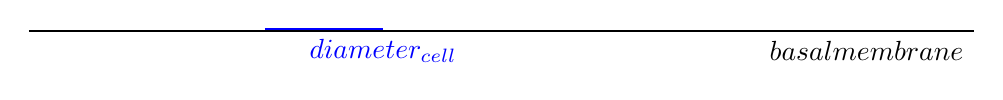
\begin{tikzpicture}[scale=3]
%%draw the edges of the cube
\draw[black,thick] (-2,0) -- (2,0)node[anchor=north east]{$basal membrane$};
\draw[blue,thick] (-1,.01) -- (-0.5,.01)node[anchor=north]{$diameter_{cell}$};
\end{tikzpicture}
\caption{considered area to spread the stem cells in two dimensions with an example of one stem cell placed on the basal membrane. Because only the x-axis is displayed we need to calculate the diameter of a cell}
\label{tikz:AreaIn2D}
\end{center}
\end{figure}


\begin{figure}[h]
\begin{center}
\begin{tikzpicture}[MyPersp,font=\large]
%%draw the edges of the cube
%\draw[pattern=north west lines, pattern color=blue] (0,0) rectangle (2,4);
\draw[pattern=north west lines, pattern color=gray] (0,0,0) -- (0,2.25,0) -- (3.25,2.25,0) -- (3.25,0,0) -- cycle;
\fill[blue] (1,1.75)   circle[radius=0.125];
 
\end{tikzpicture}
\caption{considered area to spread the stem cells in three dimensions with an example of one stem cell placed on the basal membrane. This stem cell is a circle, because for the calculation we use two dimensions}
\label{tikz:AreaIn3D}
\end{center}
\end{figure}


The following formulas calculate the amount of stem cells in two dimensions:

\begin{equation}\label{eq:Area12-2D}
A_{stem cells} = xLength * 0.12
\end{equation}
\begin{equation}\label{eq:AmounStemCell2D}
Amount_{StemCells} = \dfrac{A_{stem cells}}{diameter} 
\end{equation}
Formula \ref{eq:Area12-2D} ensures that only 12\% of the given area is used. Formula \ref{eq:AmounStemCell2D} then calculates the amount of stem cells on this given area. Since the result of the calculation is often not a whole number, the result is checked if the first decimal digit is larger or equal than 5 and then it is rounded up or down. This has a significant difference in the result, as it is displayed in table \ref{tbl:Approximation error} at page \pageref{tbl:Approximation error}.
\begin{table}
\centering
\caption{Possible approximation error by not rounding the result of formula \ref{eq:AmounStemCell2D}}
\renewcommand{\arraystretch}{1.5}
	\begin{tabularx}{\textwidth}{XXXXX}
		XLength in \SI{}{\micro\metre} & Result of $Amount_{StemCells}$ & rounded or casted result & Area used of Stem cells in \SI{}{\micro\metre} & relative used area  \\
		\hline
		200 & $\sim 2.66$ & 3 & 27 & 13.5\% \\
		
		200 & $\sim 2.66$ & 2 & 18 & 9\% 

	\end{tabularx}
	\label{tbl:Approximation error}
\end{table}

As the table displays, it is important to round the result. Otherwise there would be an approximation error which is to avoid.
\newline
For three dimensions the formulas \ref{eq:Area12-2D} and \ref{eq:AmounStemCell2D} have to be extended, because the z-axis is now also considered in the calculation of the amount of stem cells on the basal membrane. Therfore, the extended formulas for three dimensions are:
\begin{equation}\label{eq:Area12-3D}
A_{stem cells} = xLength * zLength * 0.12
\end{equation}
\begin{equation}\label{eq:AmounStemCell3D}
Amount_{StemCells} = \dfrac{A_{stem cells}}{\pi * r^{2}} 
\end{equation}
The result of formula \ref{eq:AmounStemCell3D} has to be rounded as well, otherwise the program would again include rounding errors, as it is shown in table \ref{tbl:Approximation error}. That the formulas are correct is shown with the following example. In order to keep a good overview of the results and the parameters in the formulas, the decimal digits are rounded after the third decimal digit. \newline
For a simulation with a length of \SI{200}{\micro\metre} at the x-axis and a length of \SI{50}{\micro\metre} at the z-axis, the overall area is $\SI{10000}{\micro\metre}^{2}$ and the for the stem cells reserved 12\% of the membrane are $\SI{1200}{\micro\metre}^{2}$. With an average diameter of \SI{9}{\micro\metre}, the minimum and maximum diameter of the different cells are displayed in table \ref{tab:Cell-properties} at page \pageref{tab:Cell-properties}, the result of the amount of stem cells is $\sim 18.863$ which is rounded up to 19 stem cells on an area of $\SI{10000}{\micro\metre}^{2}$.

\begin{equation}
\begin{split}
Amount_{StemCells} & = \dfrac{\SI{200}{\micro\metre} * \SI{50}{\micro\metre} * 0.12}{\pi * r^{2}} \\
					& = \dfrac{\SI{1200}{\micro\metre^{2}}}{\SI{63.617}{\micro\metre^{2}}} \\
					& \sim 18.863 \\
					& = 19
\end{split}
\end{equation}
To validate this result, the area of 19 circles with a radius of $\dfrac{\SI{9}{\micro\metre}}{2}$ has to be calculated. To then get the relative amount of stem cells on the basal membrane it is required to divide the result of $Amount_{StemCells}$ with the overall possible area of the urothel. As the calculations show, on an area with $\SI{10000}{\micro\metre}^{2}$ to draw 19 cells uses 12\% of the given area.

\begin{equation}
\begin{split}
A_{StemCells} & = 19 * \pi *  cell radius^{2} \\
					& = 19 * \pi *  \SI{4.5}{\micro\metre^{2}}  \\
					& \sim \SI{1208.728}{\micro\metre^{2}}
\end{split}
\end{equation}

\begin{equation}
\begin{split}
A_{StemCells} & = \dfrac{A_{StemCells}}{\SI{10000}{\micro\metre^{2}}} \\
				& = \dfrac{\SI{1208.728}{\micro\metre^{2}}}{\SI{10000}{\micro\metre^{2}}} \\
				& = 0.120 \\
				& = 12\%
\end{split}
\end{equation}

In the following listing the new calculation to figure out the amount of stem cells on the basal membrane at the start of the simulation is shown. The calculation is for two as well as for three dimensions modified, since both did not have a mathematical evidence.

\begin{lstlisting}[language=Python, caption= new calculation of the amount of stem cells on the basal membrane with a mathematical evidence]
    def _initCells(self, steppable):
...
        cellDiameter = self.cellTypes[2].getAvgDiameter() # cell diameter is of type float


        if self.execConfig.dimensions == 2:
            noStemCells = int(self.execConfig.xLength * 0.12 / cellDiameter)
        else:
            noStemCells = ((self.execConfig.xLength * self.execConfig.zLength) * 0.12) / (PI * (cellDiameter / 2.) ** 2)

        if noStemCells % 1 > 0.5:
            noStemCells += 1

        noStemCells = int(noStemCells)
...
\end{lstlisting}

\section{TargetVolume, Surface after Mitosis}
Mmitosis is done by \ac{CC3D}, i.e. \ac{CC3D} decides where the cell splits and calculates the volumes and the surface of the two new cells. In our program we calculate and set attributes of the new cells, e.g. the target volume or the target surface. The target volume is simply calculated by dividing the target volume of the cell before mitosis by 2. This value is applied for both new created cells. The problem with this technique is that it is possible that the cell does not split complety in the middle. Therefore, it is not possible to set the target volume of the two created cells without the knowledge of the volume of both cells. Moreover, the function 'initCellAttributes' calles the function 'setCellAttributes', in which the targetVolume of the specific cell is set to be 1 larger than the current volume. If the commands of the function 'initCellAttributes' are complete and the program is again in the below listet function, then the target volume of both cells is set to a value which has no evidence to be correct.
\begin{lstlisting}[language=Python, caption=two cells are created by mitosis where the target volume is set at a wrong place]
    def updateAttributes(self):
        parentCell = self.mitosisSteppable.parentCell
        childCell = self.mitosisSteppable.childCell

        #Has to be done this way otherwise if cell.volume is chosen than it disappears
        newVol = parentCell.targetVolume / 2

        descendents = self.model.cellTypes[parentCell.type].getDescendants()
        parentCell.type = descendents[0]
        childCell.type = descendents[1]

        # Now set the attributes for the two daughter cells:
        cellDictChild = self.getDictionaryAttribute(childCell)
        self.model.initCellAttributes(childCell, cellDictChild)
        cellDictParent = self.getDictionaryAttribute(parentCell)
        self.model.initCellAttributes(parentCell, cellDictParent)

        parentCell.targetVolume = newVol
        childCell.targetVolume = newVol

        # Register events
        self._cellLifeCycleBirth(parentCell)
        self._cellLifeCycleBirth(childCell)
		cellDictChild['colony'] = cellDictParent['colony']
\end{lstlisting}\label{lst:TargetVolumeWrongPlace}
\begin{lstlisting}[language=Python, caption=set the target volume as well as the target surface in the intended function]
    def setCellAttributes(self, cellDict, cell, lifeTimeParent):
		...
        cell.targetVolume = cell.volume + 1  # At the beginning, the target is the actual size.
        cell.targetSurface = self.execConfig.calcVoxelSurfaceFromVoxelVolume(cell.targetVolume)
        ...
\end{lstlisting}
Since \ac{CC3D} calculates the new volume of both created cells and the cell attributes are initialized and set in the functions 'initCellAttributes' and 'setCellAttributes', which is called by 'initCellAttributes', setting the target volume for both cells like it is in \ref{lst:TargetVolumeWrongPlace} is not correct. Thus, these commands are deleted and the target volume will now only be set at the function 'setCellAttributes'. There the target volume is 1 larger than the current volume, because the cells are just created. With the next \ac{MCS}, and then every \ac{MCS}, the target volume will be calculated regarding the growth per day of the specific cell type. Thus, no changes in the function 'setCellAttributes' were requirded, the actual code of the function 'updateAttributes' is the following:

\begin{lstlisting}[language=Python, caption = two cells are created\, due to mitosis]
    def updateAttributes(self):
        print 'GrowthMitosisSteppable.updateAttributes()'
        parentCell = self.mitosisSteppable.parentCell
        childCell = self.mitosisSteppable.childCell

        # return cell types based on the probability (in ****Ua) two descendents of the current cell
        descendents = self.model.cellTypes[parentCell.type].getDescendants()
        parentCell.type = descendents[0]
        childCell.type = descendents[1]

        # Now set the attributes for the two daughter cells:
        cellDictChild = self.getDictionaryAttribute(childCell)
        self.model.initCellAttributes(childCell, cellDictChild)
        cellDictParent = self.getDictionaryAttribute(parentCell)
        self.model.initCellAttributes(parentCell, cellDictParent)

        print 'parentCell.volume {} >= parentCell.targetVolue {}'.format(parentCell.volume, parentCell.targetVolume)
        print 'childCell.volume {} >= childCell.targetVolue {}'.format(childCell.volume, childCell.targetVolume)

        # Register events
        self._cellLifeCycleBirth(parentCell)
        self._cellLifeCycleBirth(childCell)
        cellDictChild['colony'] = cellDictParent['colony']
\end{lstlisting}























